\documentclass[10pt,aspectratio=169]{beamer}

% All the boilerplate is in deslides.sty
\usepackage{deslides}

\author{Ji\v{r}\'i Lebl}

\institute[OSU]{%
Oklahoma State University%
%Departemento pri Matematiko de Oklahoma {\^S}tata Universitato%
}

\title{6. Separable equations (Notes on Diffy Qs, 1.3)}

\date{}

\begin{document}

\begin{frame}
\titlepage

%\bigskip

\begin{center}
The textbook: \url{https://www.jirka.org/diffyqs/}
\end{center}
\end{frame}

\begin{frame}
Given
$y' = f(x)$ we integrate to solve: $y = \int f(x) \,dx + C$. 

\medskip
\pause

Similarly we solved $y' = f(y)$ by writing $x$ in terms of $y$.

\medskip
\pause

But the strategy doesn't work for the general $y' = f(x,y)$.

\medskip
\pause

Integrating yields
\[
y = \int f(x,y) \,dx + C .
\]

\medskip
\pause

But if the equation is so-called ``separable,'' then we can
still integrate.

\end{frame}

\begin{frame}

A differential equation is \emph{separable} if we can write it as
\[
y' = f(x)g(y) ,
\]
\pause
Using the Leibniz notation $\dfrac{dy}{dx} = f(x)g(y)$, rewrite it as
\[
\frac{dy}{g(y)} = f(x) \,dx .
\]
\pause
Integrate both sides:
\[
\int \frac{dy}{g(y)} = \int f(x) \,dx + C .
\]
\pause
Solve for $y$ (if you can).

\end{frame}

\begin{frame}

\textbf{Example:}
Consider
$y' = xy$.

\medskip
\pause

$y=0$ is a solution, so remember that and assume $y\not= 0$ from now.

\medskip
\pause

Write:
\qquad $\displaystyle \frac{dy}{dx} = xy$
\quad as \quad
$\displaystyle \frac{1}{y}\, dy = x \, dx$
\pause
\qquad Integrate:
$\displaystyle
\int \frac{dy}{y} = \int x\,dx + C$

\medskip
\pause

\thus
\quad
$\displaystyle
\ln \, \lvert y\rvert = \frac{x^2}{2} + C$
\pause
\wthus
$\displaystyle \lvert y \rvert = e^{\frac{x^2}{2} + C}
\pause
 = e^C e^{\frac{x^2}{2}}$

\medskip
\pause

$e^C$ is an arbitrary positive constant.

\pause
Because of the absolute value we could replace it with a negative.

\pause
And $y=0$ is also a solution.

\medskip
\pause

So the general solution is \quad $\displaystyle y = D e^{\frac{x^2}{2}}$
\quad ($D$ a constant).

\medskip
\pause

Check:
$\displaystyle
y' \pause = D x e^{\frac{x^2}{2}} \pause = x \left( D e^{\frac{x^2}{2}}
\right) \pause = xy$.
\qquad
{\Large\checkmark}
\end{frame}

\begin{frame}
It appears as if we are integrating with two different variables.

\medskip
\pause

So why does it work?

\medskip
\pause

Note that $y=y(x)$ and $\dfrac{dy}{dx}$ are functions of $x$.

\medskip
\pause

Write
\quad
$\displaystyle \frac{dy}{dx} = f(x)g(y)$
\quad
as
\quad
$\displaystyle
\frac{1}{g(y)}\,\frac{dy}{dx} = f(x)$.

\medskip
\pause

Now integrate both sides wrt $x$:
\quad
$\displaystyle
\int \frac{1}{g(y)}\,\frac{dy}{dx} \,dx = \int f(x) \,dx + C$.

\medskip
\pause

Substitution formula from calculus says
\quad $\displaystyle
\int \frac{1}{g(y)}\,dy = \int f(x) \,dx + C$.
\quad
{\Large\checkmark}

\end{frame}

\begin{frame}
Solving for $y$ can be difficult.

\medskip
\pause

\textbf{Example:}
Consider \quad
$\displaystyle
y' = \frac{xy}{y^2+1}$.
\qquad
\pause
$y=0$ is a solution, so assume $y\not= 0$ from now.

\medskip
\pause

Separate variables:
\quad
$\displaystyle
\frac{y^2+1}{y}\,dy = \left(y+\frac{1}{y}\right)\,dy = x\,dx$.
\qquad
\pause
Integrate:
\quad
$\displaystyle
\frac{y^2}{2} + \ln \, \lvert y \rvert = \frac{x^2}{2} + C$,

\medskip
\pause

Simplify
\quad
$\displaystyle
y^2 + 2 \ln \, \lvert y\rvert = x^2 + D$
\quad ($D=2C$).

\medskip
\pause

We can't solve for $y$ in a ``nice'' expression.

\pause

Just leave it as is.
\pause
It is called an \emph{implicit solution}.

\medskip
\pause

We can still check that it satisfies the equation.
\pause

Differentiate remembering that $y=y(x)$ is a function of $x$:

\medskip
\pause

\quad
$\displaystyle
y'\left(2y + \nicefrac{2}{y}\right) = 2x$
\pause\wthus
$\displaystyle
y'\left(2y + \nicefrac{2}{y}\right)\frac{y}{2(y^2+1)} = 2x\frac{y}{2(y^2+1)}$
\pause\wthus
$\displaystyle
y' = \frac{xy}{y^2+1}$
\quad
{\Large\checkmark}

\medskip
\pause

The general solution is
\begin{equation*}
y^2 + 2 \ln \, \lvert y \rvert = x^2 + C, \qquad \text{and} \qquad y=0.
\end{equation*}
\pause
Solutions such as $y=0$ are sometimes called \emph{singular solutions}.


\end{frame}

\begin{frame}
Computing values of $y$ given $x$ is tricky.
\pause
You might even get multiple values.

\medskip
\pause

Often one uses computers to find values.

\medskip
\pause

Here is what the set of points $(x,y)$ satisfying 
$y^2+2\ln|y|=x^2$ looks like:

\begin{center}
\includegraphics[width=3in]{../figures/implicitsols}
\end{center}

\medskip
\pause

The initial condition tells you which solution to take.
\pause
E.g., the top curve satisfies $y(1)=1$.

\end{frame}

\begin{frame}
A couple more examples of separable equations:

\medskip
\pause

\textbf{Example:}
Solve \quad $x^2y' = 1 - x^2+y^2 - x^2y^2$, \quad $y(1) = 0$.

\medskip
\pause

Factor:
\quad
$\displaystyle
x^2y' = (1 - x^2)(1+y^2)$.

\medskip
\pause

Separate variables, integrate, and solve for $y$:

\medskip
\pause

\quad
$\displaystyle
\frac{y'}{1+y^2} = \frac{1 - x^2}{x^2}$
\pause
\wthus
$\displaystyle
\frac{y'}{1+y^2} = \frac{1}{x^2} - 1$
\pause
\wthus
$\displaystyle
\operatorname{arctan} (y) = \frac{-1}{x} - x + C$

\medskip
\pause

\wthus
\quad
$\displaystyle
y = \tan \left(\frac{-1}{x} - x + C\right)$

\medskip
\pause

Solve for IC:
\quad
$0 = \tan(-2+C)$
\pause
\wthus
$C=2$ \pause \quad (or $C = 2 + \pi$, or $C = 2 + 2\pi$, etc.)

\medskip
\pause

The particular solution we seek is
\quad
$\displaystyle
y = \tan \left(\frac{-1}{x} - x + 2 \right)$.

\end{frame}

\begin{frame}

\textbf{Example:}
Bob wants to drink coffee at 60${}^\circ$C.

\pause
Initially (time $t=0$), the temperature was 89${}^\circ$C.

\pause
One minute later, the temperature was 85${}^\circ$C.

\pause
The room has temperature 22${}^\circ$C.

\pause
When can Bob start drinking?

\medskip
\pause

Let $T =$ the temperature of the coffee in ${}^\circ$C.

\pause
Let $A =$ the ambient temperature in ${}^\circ$C

\medskip
\pause

Newton's law of cooling states \qquad
$\dfrac{dT}{dt} = k(A-T)$ \quad for some $k > 0$.

\medskip
\pause

We have $A=22$, $T(0)=89$, $T(1)=85$.

\medskip
\pause

Separate variables, integrate (note that $T-A > 0$):

\medskip
\pause

\quad
$\displaystyle
\frac{1}{T-A} \, \frac{dT}{dt} = -k$
\pause
\wthus
$\displaystyle
\ln (T-A) = -kt + C$
\pause
\wthus
$\displaystyle
T-A = D\, e^{-kt}$
\pause
\wthus
$\displaystyle
T = A + D\, e^{-kt}$

\medskip
\pause

\wthus
$T = 22 + D\, e^{-kt}$

\medskip
\pause

First condition:
\quad
$89 = T(0) \pause = 22 + D$
\pause
\wthus 
$D = 67$
\pause
\wthus $T = 22 + 67\, e^{-kt}$

\medskip
\pause

Second condition
\quad
$85 = T(1) \pause
= 22 + 67\, e^{-k}$
\pause
\wthus
$k = - \ln \frac{85-22}{67} \approx 0.0616$

\end{frame}

\begin{frame}
So approximately \quad $T = 22 + 67 e^{-0.0616t}$

\medskip
\pause

Solve $T=60$ for time $t$:
\quad
$60 = 22 + 67 e^{-0.0616t}$
\pause
\wthus
$t = - \frac{\ln \frac{60-22}{67}}{0.0616} \pause \approx 9.21$ minutes.

\medskip
\pause

Bob can start drinking a little over 9 minutes from when the coffee was
made.

\begin{center}
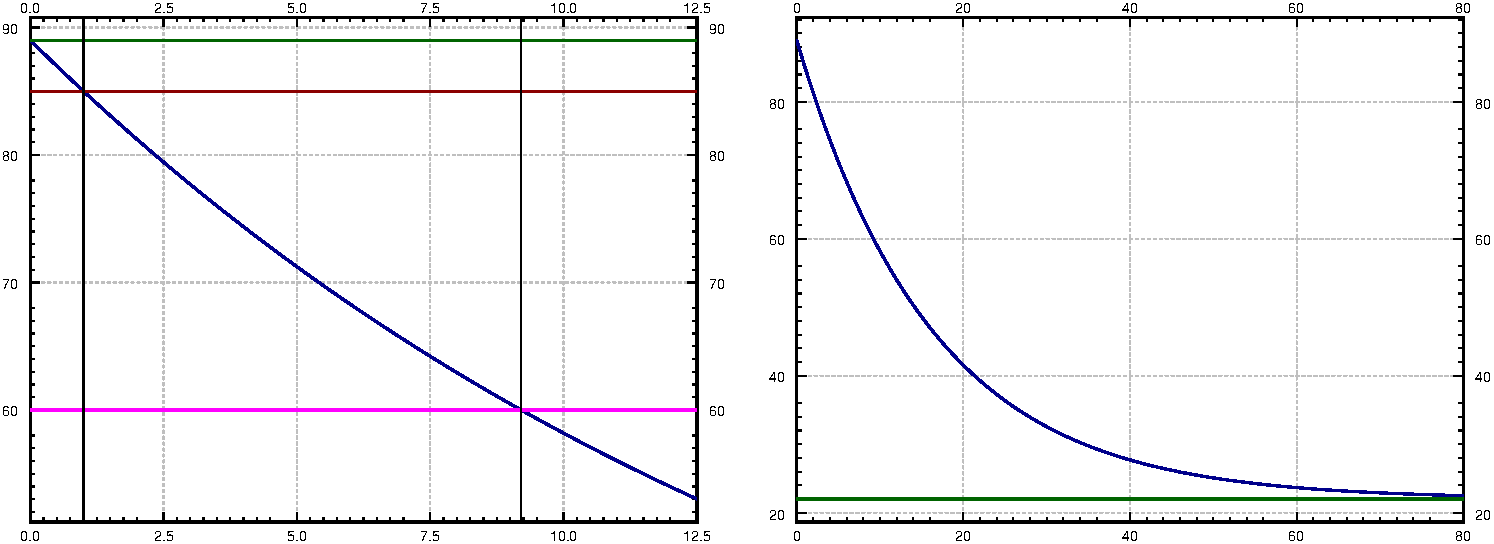
\includegraphics[width=5in]{../figures/coffeefig-1-2}
\end{center}

Graphs of the coffee temperature function $T(t)$ over different time frames.

89, 85, 60 lines are marked on the left, and $T=A$ line is marked on the
right.

\end{frame}

\begin{frame}

\textbf{Example:}
Find the general solution to $y' = \frac{-xy^2}{3}$.

\medskip
\pause

$y=0$ is a solution (a singular solution).

\medskip
\pause

Assume $y \not= 0$ and solve:

\medskip
\pause

\quad
$\displaystyle
\frac{-3}{y^2} y'  = x$
\pause
\wthus
$\displaystyle
\frac{3}{y} = \frac{x^2}{2} + C$
\pause
\wthus
$\displaystyle
y = \frac{3}{\nicefrac{x^2}{2} + C}
= \frac{6}{x^2 + 2C}
$

\medskip
\pause

The general solution is
\[
y = \frac{6}{x^2 + 2C} \qquad \text{and} \qquad y=0 .
\]

\end{frame}

\end{document}
